%\documentclass{beamer}
\documentclass[handout]{beamer}

\mode<presentation>
{
 \usetheme{Madrid}
 \usecolortheme{beaver}
 \setbeamercovered{invisible}
}
\beamertemplatenavigationsymbolsempty
\setbeamertemplate{footline}[frame number]{}
\setbeamertemplate{blocks}[shadow=true]

% packages
\hypersetup{hidelinks}
\usepackage{placeins}
\usepackage[format=plain,
            labelfont={bf,it},
            textfont=it]{caption}
\setlength{\captionmargin}{0.3in}
\usepackage{mathtools}
\usepackage{amsthm}
\usepackage{amssymb}
\usepackage{cancel}
\usepackage[italicdiff]{physics}
% \usepackage{tocloft}
\usepackage{dsfont}
\usepackage{thmtools}
\usepackage{graphicx}
% \usepackage{longtable}

\usepackage{tikz}
\usetikzlibrary{bayesnet}

\setlength{\marginparwidth}{0.75in}

\allowdisplaybreaks

% paper-specific
\renewcommand{\vec}{\mathrm{vec}}
\newcommand{\proj}{\mathrm{proj}}

\newcommand\numberthis{\addtocounter{equation}{1}\tag{\theequation}}

\newcommand{\m}[1]{\begin{pmatrix}#1\end{pmatrix}}  % a matrix or vector
\newcommand{\sm}[1]{\begin{psmallmatrix}#1\end{psmallmatrix}}
\newcommand{\f}[1]{\frac{\StrBefore{#1}{/}}{\StrBehind{#1}{/}}} % easier fractions
\renewcommand{\sf}[1]{\tfrac{\StrBefore{#1}{/}}{\StrBehind{#1}{/}}}
\newcommand{\half}{\frac{1}{2}}
\newcommand{\thalf}{\tfrac{1}{2}}
\newcommand{\third}{\frac{1}{3}}
\newcommand{\quarter}{\frac{1}{4}}

\newcommand{\eps}{\varepsilon}
\newcommand{\clos}[1]{\overline{#1}}
\newcommand{\conj}[1]{\overline{#1}}
\newcommand{\dfeq}{\coloneqq}

\let\sp\undefined
\DeclareMathOperator{\id}{id}
\DeclareMathOperator*{\argmax}{arg\,max}
\DeclareMathOperator*{\argmin}{arg\,min}

\DeclareMathOperator{\E}{\mathbb{E}}
\let\Pr\undefined
\DeclareMathOperator{\Pr}{\mathbb{P}}
\newcommand{\indep}{\mathbin{\perp\!\!\!\!\!\:\perp}}
\newcommand{\notindep}{\mathbin{\perp\!\!\!\!\not\!\:\perp}}
\newcommand{\gvn}{\;\middle|\;}
\newcommand{\R}{\ensuremath{\mathbb{R}}}
\newcommand{\F}{\ensuremath{\mathcal{F}}}
\newcommand{\B}{\ensuremath{\mathcal{B}}}
\newcommand{\ind}{\mathds{1}}
\newcommand{\iid}{\mathrel{\stackrel{iid}{\sim}}}
\newcommand{\rv}{random variable}
\newcommand{\rvs}{random variables}
\newcommand{\iidt}{independent and identically distributed}
\newcommand{\cvp}{\xrightarrow{\:p\,}}
\newcommand{\cvw}{\xrightarrow{\,w\,}}
\newcommand{\cvd}{\xrightarrow{\,d\,}}
\newcommand{\cvas}{\xrightarrow{\;\!a.s.\:\!}}
\newcommand{\cvlp}[1]{\xrightarrow{\;\!L^{#1}\,\!}}

\DeclareMathOperator{\Var}{\mathbb{V}}
\DeclareMathOperator{\Cov}{Cov}
\DeclareMathOperator{\Corr}{Corr}
\DeclareMathOperator{\Unif}{Unif}
\DeclareMathOperator{\Expo}{Expo}
\DeclareMathOperator{\Cauchy}{Cauchy}
\DeclareMathOperator{\logit}{logit}
\newcommand{\Inv}{\mathrm{Inv-}}
\newcommand{\Pois}{\mathrm{Pois}\qty}
\newcommand{\Beta}{\mathrm{Beta}\qty}
\newcommand{\Categorical}{\mathrm{Cat}}
\newcommand{\Dirichlet}{\mathrm{Dir}\qty}
\newcommand{\Gam}{\mathrm{Gamma}\qty}
\newcommand{\Wei}{\mathrm{Wei}\qty}
\newcommand{\Hyper}{\mathrm{HGeom}\qty}
\newcommand{\Binom}{\mathrm{Bin}\qty}
\newcommand{\NBinom}{\mathrm{NBin}\qty}
\newcommand{\Multinom}{\mathrm{Multinom}\qty}
\newcommand{\Bern}{\mathrm{Bern}\qty}
\newcommand{\Bernoulli}{\mathrm{Bernoulli}\qty}
\newcommand{\Norm}{\mathcal{N}\qty}
\newcommand{\MVNorm}[1][]{\mathcal{N}_{#1}\qty}
\DeclareMathOperator{\Student}{Student-\mathit{t}}

\DeclarePairedDelimiter\br{\langle}{\rangle}
\DeclarePairedDelimiter\ceil{\lceil}{\rceil}
\DeclarePairedDelimiter\floor{\lfloor}{\rfloor}
\DeclarePairedDelimiter\round{\lceil}{\rfloor}
\DeclarePairedDelimiter\set{\{}{\}}

\DeclareMathOperator{\sgn}{sgn}
\DeclareMathOperator{\diag}{diag}
\providecommand{\norm}[1]{\lVert#1\rVert}

\newcommand{\cS}{\mathcal{S}}
\newcommand{\cR}{\mathcal{R}}
\newcommand{\cG}{\mathcal{G}}
\newcommand{\cZ}{\mathcal{Z}}
\newcommand{\cX}{\mathcal{X}}
\newcommand{\cY}{\mathcal{Y}}
\newcommand{\cW}{\mathcal{W}}
\newcommand{\cI}{\mathcal{I}}


%%%%%%%%%%%%%%%%%%%%%%%%%%%%%%%%%%%%%%%%%%%%%%%%%%%%%%%%%%%%%%%%%%%%%%

% If you wish to uncover everything in a step-wise fashion, uncomment
% the following command:
\beamerdefaultoverlayspecification{<+->}


\newcommand{\tit}{\bf Estimating Racial Disparities when\\ Race is Not Observed}

% == titles
\title[]{\tit}

\institute[Harvard]{\large Harvard University }

\date{Interdisciplinary Seminar on Social Science Methodology \\
  Interdisciplinary Seminar in Quantitative Methods,\\  University of Michigan\\
  March 10, 2023 \\  \vspace{.25in} Joint work with
  Cory McCartan, Jacob Goldin, and Daniel E. Ho } 


\author[Kosuke Imai]{\large Kosuke Imai }


% == document begins
\begin{document}

%%% Title
\frame{\titlepage}

%%% Table of Contents
% \frame{\tableofcontents}

%%% Main Contents

\section{Introduction}

\begin{frame}

  \frametitle{Motivation}

  \begin{itemize}
  \item Importance of racial disparity estimation in many fields:\\
    public health, employment, voting, criminal justice, taxation,
    housing, lending, and internet technology

    \vfill
  \item But, often individual race is not available
    \begin{itemize}
    \item law may prohibit collection of information about race
      (e.g., Equal Credit Opportunity Act)
    \item agencies and companies may not wish to collect such information
    \end{itemize}
    \vfill
  \item How should we estimate racial disparities when race is not
    observed?
    \begin{itemize}
    \item Standard methods use BISG (Bayesian Improved Surname
      Geocoding)
    \item But, it has been shown that they are likely to yield biased estimates
    \end{itemize}

  \item Can we improve the standard methods and eliminate their bias? 
  \end{itemize}

\end{frame}


\begin{frame}

  \frametitle{Executive Order 13985: {\small Advancing Racial Equity and Support for Underserved Communities through the Federal Government}}

  \begin{itemize}
  \item \alert{Sec. 4.  Identifying Methods to Assess Equity}.  (a)
    The Director of the Office of Management and Budget (OMB) shall,
    in partnership with the heads of agencies, study methods for
    assessing whether agency policies and actions create or exacerbate
    barriers to full and equal participation by all eligible
    individuals.  The study should aim to identify the best methods,
    consistent with applicable law, to assist agencies in assessing
    equity with respect to race, ethnicity, religion, income,
    geography, gender identity, sexual orientation, and disability.

    \vfill
  \item \alert{Sec. 5.  Conducting an Equity Assessment in Federal
      Agencies.}  The head of each agency, or designee, shall, in
    consultation with the Director of OMB, select certain of the
    agency's programs and policies for a review that will assess
    whether underserved communities and their members face systemic
    barriers in accessing benefits and opportunities available
    pursuant to those policies and programs.
  \end{itemize}

\end{frame}

\begin{frame}

  \frametitle{Overview of the Talk}

  \begin{enumerate}
  \item Existing methods are likely to be biased
    \begin{itemize}
    \item BISG predictions are typically accurate and well calibrated
    \item Still, estimates of racial disparities based on them can be biased
    \item This is because race affects many aspects of our society
    \end{itemize}
    \bigskip
  \item \alert{BIRDiE} (Bayesian Instrumental Regression for Disparity
    Estimation) 
    \begin{itemize}
    \item New and more credible identification assumption
    \item Flexible model allows for various racial disparity estimands
    \item Sensitivity analysis for potential violation of the
      assumption
    \item Open-source software package \alert{birdie} available
    \end{itemize}
    \begin{flushright}
      \vspace{-.5in}
      
\includegraphics[scale=0.165]{../man/figures/logo.png}
     \end{flushright}
  \item Empirical validation
    \begin{itemize}
    \item North Carolina voter file where self-reported race is
      observed
    \item Estimates of racial differences in party registration
    \item BIRDiE yields much smaller bias than the standard methods
    \item Results are robust to potential violation of assumptions
    \end{itemize}
  \end{enumerate}

\end{frame}


\begin{frame}

\frametitle{The Setup}

\begin{itemize}
\item Data
  \begin{itemize}
  \item $Y_i$: outcome of interest 
  \item $R_i$: (unobserved) race
  \item $S_i$: surname
  \item $G_i$: residence location
  \item $X_i$: other Census variables (optional)
  \item $W_i$: covariates of interest
  \end{itemize}
\item Census data
  \begin{itemize}
  \item $\Pr(G_i = g, R_i = r, X_i = x)$
  \item $\Pr(R_i = r, S_i =s)$ for frequently occurring surnames
  \end{itemize}

  \vfill
\item Regression estimands
  \begin{itemize}
  \item $\Pr(Y_i = y \mid R_i = r)$: short regression
  \item $\Pr(Y_i = y \mid R_i = r, X_i =x)$: long regression 
  \end{itemize}

\item Racial disparity estimands
  \begin{itemize}
  \item $\Pr(Y_i =y \mid R_i = r) - \Pr(Y_i = y \mid R_i = r^\prime)$ for $r
    \ne r^\prime$
  \item $\Pr(Y_i = y \mid R_i = r, W_i = w) - \Pr(Y_i = y \mid R_i = r^\prime, W_i = w)$
  \end{itemize}

\end{itemize}
  
\end{frame}

\begin{frame}

  \frametitle{Standard Estimation Methods}
 
\begin{enumerate}
\item Predict race via \alert{BISG} (or its variant)
  \begin{itemize}
  \item Assumption: $G_i \indep  S_i \mid R_i$
  \item Bayes rule:
    \begin{align*}
      \hat{P}_{ir} \ & = \ \Pr(R_i = r \mid G_i = g, S_i = s) \\
      \onslide<3->{& = \ \frac{\Pr(S_i =s\mid
      \alert{G_i =g}, R_i = r)\Pr(G_i =g, R_i =r)}{\sum_{r^\prime} \Pr(S_i =s\mid
          \alert{G_i =g}, R_i = r^\prime)\Pr(G_i =g, R_i =r^\prime)}} \\
      \onslide<4->{& = \ \frac{\Pr(S_i =s\mid
       R_i = r)\Pr(G_i =g, R_i =r)}{\sum_{r^\prime} \Pr(S_i =s\mid
       R_i = r^\prime)\Pr(G_i =g, R_i =r^\prime)}}
    \end{align*}
  \item<5-> With covariates: $(G_i, X_i) \indep S_i \mid R_i$
  \item<6-> {\sc wru} software package {\scriptsize (Imai and Kahna 2016)}
  \end{itemize}
  \vfill
\item<7-> Estimate racial disparities $\mu_{Y\mid R}(y \mid r) = \Pr(Y_i = y \mid R_i = r)$
  \begin{itemize}
  \item<8-> \alert{weighting}:
    $$\hat\mu_{Y\mid R}^{\text{wtd}}(y \mid r) \ = \ \frac{\sum_i \mathbf{1}\{Y_i = y\}\hat{P}_{ir} }{\sum_i \hat{P}_{ir}}$$
  \item<9-> \alert{thresholding}: use the racial group with the largest
    probability as imputed race
  \end{itemize}
\end{enumerate}

\end{frame}

\begin{frame}

  \frametitle{BISG Prediction Works Reasonably Well {\scriptsize (Imai
      et al. 2022. {\it Sci. Adv.})}}

  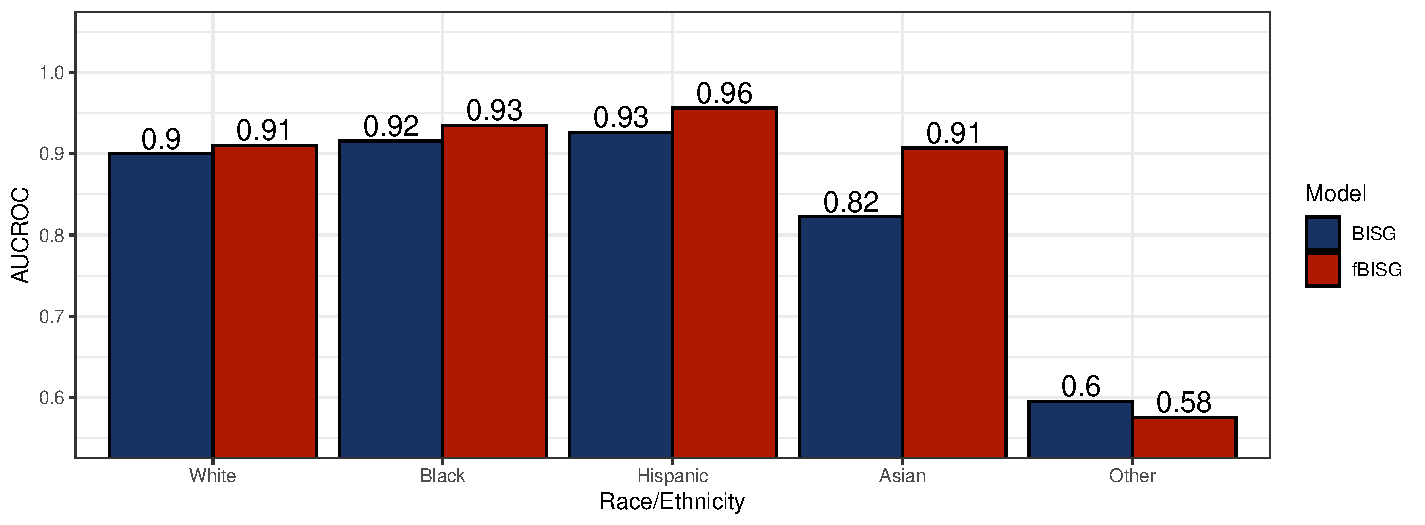
\includegraphics[width=\textwidth]{figs/AUCROC_Surnames.pdf}\\
  \onslide<2->{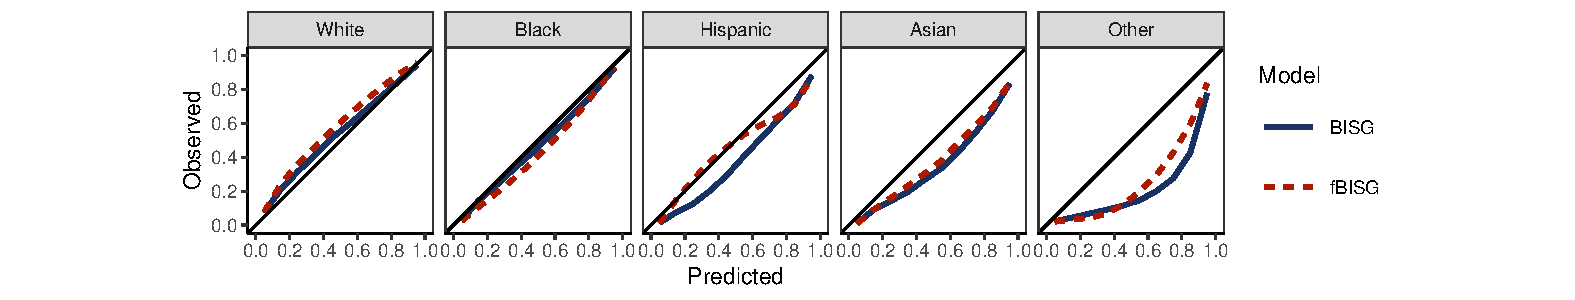
\includegraphics[width=1.2\textwidth, trim = 100 0 0 0, clip]{figs/Calibration_Surnames.pdf}}

\end{frame}

\begin{frame}

  \frametitle{Good Race Prediction Can Bias Racial
    Disparity Estimates}

  \begin{columns}
    \begin{column}{0.575\textwidth}
      \begin{itemize}
      \item Bias of the weighted estimator {\scriptsize (Chen {\it et
            al.} 2019)}
        \begin{align*}
          & \hat\mu_{Y\mid R}^{\text{wtd}}(y \mid r) - \Pr(Y_i = y
            \mid R_i = r) \\
= & - \frac{\E[\text{Cov}(\mathbf{1}\{Y_i = y\}, \mathbf{1}\{R_i = r\}\mid G_i,
          X_i, S_i)]}{\Pr(R_i = r)}
          \end{align*}

          \vfill
        \item Required assumption: $$Y_i \indep R_i \mid G_i, S_i, X_i$$
          \vfill
     \item Problem: race affects many aspects of the society
      \end{itemize}
    \end{column}
    \begin{column}{0.425\textwidth}
      \tikzstyle{main node}=[circle,draw,font=\sffamily\Large\bfseries]
      \tikzstyle{sub node}=[circle,draw,dashed,font=\sffamily\Large\bfseries]
      \hspace{-.2in}\begin{tikzpicture}[->,>=stealth',shorten >=1pt,auto,node distance=2.6cm,thick]
        
        \node[main node] (G) {$G$};
        \node[main node] (Y) [right of=G] {$Y$};
        \node[main node] (S) [below left=1.3cm and 1.3cm of Y] {$S$};
        \node[sub node] (R) [below left=0.8cm and 0.8cm of S] {$R$};
        \node[main node] (X) [below of=Y] {$X$};
        
        \path[every node/.style={font=\sffamily\small}]
        (R) edge node  {} (G)
        (R) edge node  {} (X)
        (S) edge node  {} (Y)
        (R) edge node  {} (S)
        (G) edge node  {} (X)
        (G) edge node  {} (Y)
        (X) edge node  {} (Y);
    \end{tikzpicture}
  \end{column}
  \end{columns}

\end{frame}

\begin{frame}

\frametitle{New Identification Strategy}


  \begin{columns}
    \begin{column}{0.425\textwidth}
      \tikzstyle{main node}=[circle,draw,font=\sffamily\Large\bfseries]
      \tikzstyle{sub node}=[circle,draw,dashed,font=\sffamily\Large\bfseries]
   \begin{tikzpicture}[->,>=stealth',shorten >=1pt,auto,node distance=2.5cm,thick]
    
        \node[main node] (G) {$G$};
        \node[sub node] (R) [below of=G] {$R$};
        \node[main node] (S) [below left=0.5cm and 0.5cm of R] {$S$};
        \node[main node] (Y) [right of=G] {$Y$};
        \node[main node] (X) [below of=Y] {$X$};
        
        \path[every node/.style={font=\sffamily\small}]
        (R) edge node  {} (G)
        (R) edge node  {} (X)
        (R) edge node  {} (Y)
        (R) edge node  {} (S)
        (G) edge node  {} (X)
        (G) edge node  {} (Y)
        (X) edge node  {} (Y);
        
        %\path[every node/.style={font=\sffamily\small}, <->]
        %(G) edge [dashed, bend right] node  {} (S)
        %(X) edge [dashed, bend left] node  {} (S);
    \end{tikzpicture}
  \end{column}
   \begin{column}{0.575\textwidth}
      \begin{itemize}
        \item<2-> Required assumption: $$Y_i \indep S_i \mid G_i, R_i, X_i$$

        \item Surname as a proxy for race
        \item Race can directly or indirectly affects the outcome

          \medskip
        \item Potential violations:
          \begin{itemize}
          \item name-based discrimination
          \item coarse racial categories
          \end{itemize}
        \item Anonymous application
      \end{itemize}
    \end{column}
  \end{columns}
  
\end{frame}


\begin{frame}

  \frametitle{Surname as a High-dimensional Instrument}

  \begin{itemize}
  \item Identification {\scriptsize (Kuroki and Pearl, 2014)}
    {\small\begin{align*}
     & \overbrace{\Pr(Y_i=y\mid G_i=g, X_i=x, S_i=s)}^{\text{observed data}} \\
    = & \sum_{r\in\mathcal{R}} \underbrace{\alert{\Pr(Y_i=y\mid R_i=r, G_i=g,
        X_i=x)}}_{\text{unknown parameters}}\ \underbrace{\Pr(R_i=r\mid
        G_i=g, X_i=x, S_i=s)}_{\text{BISG probability}}
           \end{align*}}
    \vspace{-.2in}
         \begin{itemize}
         \item $(|\mathcal{Y}|-1)\times|\mathcal{G}|\times|\mathcal{X}|\times|\mathcal{S}|$ equations
         \item
           $(|\mathcal{Y}|-1)\times|\mathcal{G}|\times|\mathcal{X}|\times|\mathcal{R}|$
           unknown parameters
         \end{itemize}
         \vfill
       \item OLS estimator {\scriptsize (see also Fong and Tyler, 2021)}:
         $$
    \hat{\vb*\mu}^{(\text{ols})}_{Y\mid RGX}(y\mid \cdot, g,x) 
    =  (\hat{\vb P}_{\cI(xg)}^\top \hat{\vb P}_{\cI(xg)})^{-1}\hat{\vb P}_{\cI(xg)}\,\ind\{{\vb Y}_{\cI(xg)} = y\},
    $$
    \vspace{-.2in}
    \begin{itemize}
    \item compute this for each $g$ and $x$, and aggregate
    \item unbiased estimate of $\Pr(Y_i= y \mid R_i = r)$
    \item ignores the fact that $\Pr(Y_i= y \mid R_i = r, G_i
      = g, X_i = x)$ is probability
  \end{itemize}
  \end{itemize}

\end{frame}

\begin{frame}

  \frametitle{BIRDiE {\small (Bayesian Instrumental Regression for Disparity
    Estimation)}}

\begin{itemize}
\item Flexible and scalable probabilistic model that integrates BISG 

\item Posterior:
    $$\pi(\Theta, \vb R\mid \vb Y, \vb G, \vb X, \vb S)
    \ \propto \ \pi(\Theta)\prod_{i=1}^N \underbrace{\pi(Y_i\mid R_i,
      G_i, X_i, \Theta)}_{\text{complete-data model}}
            \underbrace{\pi(R_i\mid G_i, X_i, S_i)}_{\text{BISG prob. } \hat{P}_{ir}}$$
\item Models: 
  \begin{enumerate}
  \item Complete-pooling:
$$Y_i\mid R_i, G_i, X_i, \Theta \sim \Categorical_{\cY}(\vb*\theta_{R_i}), \quad
        \vb*\theta_r \iid \Dirichlet(\vb*\alpha)$$
  \item Saturated (no pooling):
$$Y_i\mid R_i, G_i, X_i, \Theta \sim \Categorical_{\cY}(\vb*\theta_{R_iG_iX_i}), \quad
        \vb*\theta_{rgx} \iid \Dirichlet(\vb*\alpha)$$
      \item Partial pooling (mixed effects): $\vb W$ group-level
        covariates, $\vb Z=(X,G)$
        \begin{align*}
    Y_i\mid R_i, G_i, X_i, \Theta &\sim
                                    \Categorical_{\cY}(g^{-1}(\vb*\mu_{rgx})), \quad
    \mu_{rgxy} = \vb W\vb*\beta_{ry} + \vb Z\vb u_{ry} \\
    \quad \vb u_{ry}\mid \phi_{ry} &\sim \Norm(0,
                                     \Sigma(\vb*\phi_{ry})), \quad
    \vb*\beta_{ry} \iid f_\beta, \quad \vb*\phi_{ry} \iid f_\phi
        \end{align*}
        \vspace{-.2in}
  \end{enumerate}

  
\end{itemize}

\end{frame}


\begin{frame}

  \frametitle{Computation}

  \begin{enumerate}
  \item Small samples: \alert{direct inference}
$$
    \pi(\Theta\mid \vb Y, \vb G, \vb X, \vb S)
    \propto \pi(\Theta) \prod_{i=1}^N \sum_{r\in\cR} \pi(Y_i\mid 
    r, G_i, X_i, \Theta)\hat{P}_{ir}
    $$
    \begin{itemize}
    \item low-dimensional parameter space, MCMC is applicable (e.g.,
      Stan)
    \item but it is not scalable
    \end{itemize}
    
  \item Large samples: \alert{EM algorithm}
    \begin{itemize}
    \item E-step: update race probability (improvement upon BISG prob.)
      $$\tilde{P}_{ir\mid Y}^{(t)}
    = \frac{\pi(Y_i\mid r, G_i,, X_i, \Theta^{(t)}) \hat P_{ir}}{
        \sum_{r'\in\cR} \pi(Y_i\mid r', G_i,, X_i, \Theta^{(t)}) \hat P_{ir'} }$$
    \item M-step: maximize each $(y,x,g)$ group separately
      $$\log \pi(\Theta^{(t+1)}) + \sum_{r\in\cR}\sum_{y\in\cY}\sum_{x\in\cX}\sum_{g\in\cG} 
        \log \pi(y\mid r, g, x, \Theta^{(t+1)}) 
        \qty(\sum_{i\in\cI(yxg)} \tilde{P}_{ir\mid Y}^{(t)}) $$
    \end{itemize}

  \end{enumerate}

\end{frame}

\begin{frame}

  \frametitle{Additional Explanatory Variables}

  \begin{itemize}
  \item Long regression: $\Pr(Y_i  = y \mid R_i = r, W_i = w)$ where
    $W_i$ is not part of $(X_i, G_i)$
\vfill
  \item Two strategies:
    \begin{enumerate}
    \item Joint modeling: $\Pr(Y_i, W_i \mid R_i)$
    \item Iterative modeling: fit $\Pr(W_i \mid R_i)$ first and then use the
      updated race probability to fit $\Pr(Y_i \mid W_i, R_i)$
    \end{enumerate}
\vfill
\item Both approaches require:
   $$W_i\indep S_i\mid R_i,G_i,X_i \qand
   Y_i\indep S_i\mid W_i,R_i,G_i,X_i$$
   or equivalently
   $$(Y_i, W_i)\indep S_i\mid R_i,G_i,X_i$$
   \vspace{-.4in}
  \end{itemize}

\end{frame}

\begin{frame}

  \frametitle{Sensitivity Analysis}

  \begin{itemize}
  \item Potential violation of the key identifying assumption
    \begin{itemize}
    \item name-based discrimination
    \item racial category is too coarse
    \end{itemize}

  \item Suppose we can have information about finer ethnic groups
    $$f:\cS\to\R^d,\  d\ll|\cS|$$
    \begin{itemize}
    \item $f(\text{Imai}) = \text{Japanese}$,  $f(\text{McCartan}) =
      \text{Irish}$, etc.
    \item Assume instead
      $$Y_i\indep S_i\mid f(S_i),R_i,G_i,X_i$$
    \end{itemize}

  \item 1930 Census provides 22 groups
    \begin{itemize}
    \item Anglosphere and Black surname (third-or-more generation
      Whites and Blacks): Smith, Williams, Brown,
      ...
    \item First wave European immigration (German, Nordic, and Irish): Burns, Olson, Wagner, ...
    \item East Asian (Chinese, Japanese, Korean), South Asian
      (Indian, Southwest Asian),
      Southeast Asian and Pacific (Vietnamese, Filipino)
    \item Non-Cuban Hispanic (Mexican, Latin American), Cuban 
    \end{itemize}
 \end{itemize}


\end{frame}

\begin{frame}

  \frametitle{Empirical Validation}

  \begin{itemize}
  \item 2022 North Carolina voter file: 5.8 millon voters with
    self-reported race
  \item Subset 1 million voters $\rightsquigarrow$ negligible sampling
    uncertainty

    \vfill
  \item Focus on party registration

  \end{itemize}
  \onslide<4->{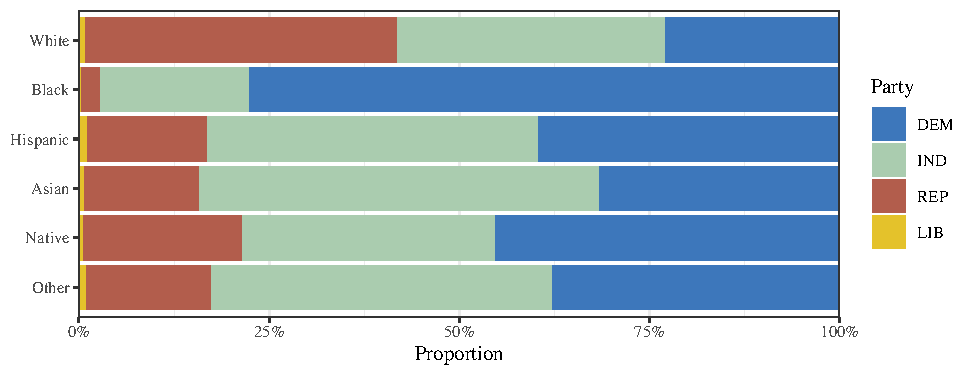
\includegraphics[width=\textwidth]{../paper/figures/nc_overview.pdf}}

\end{frame}

\begin{frame}

  \frametitle{Estimates of Racial Disparity in Party Registration}

  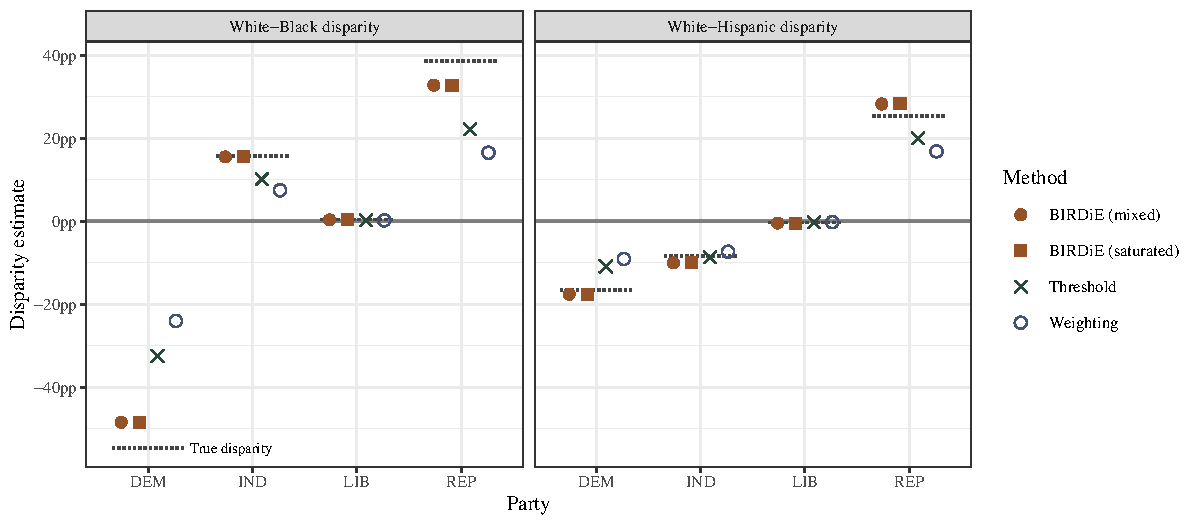
\includegraphics[width=\textwidth]{../paper/figures/nc_disp.pdf}


\end{frame}


\begin{frame}

  \frametitle{Total Variation Distance}

  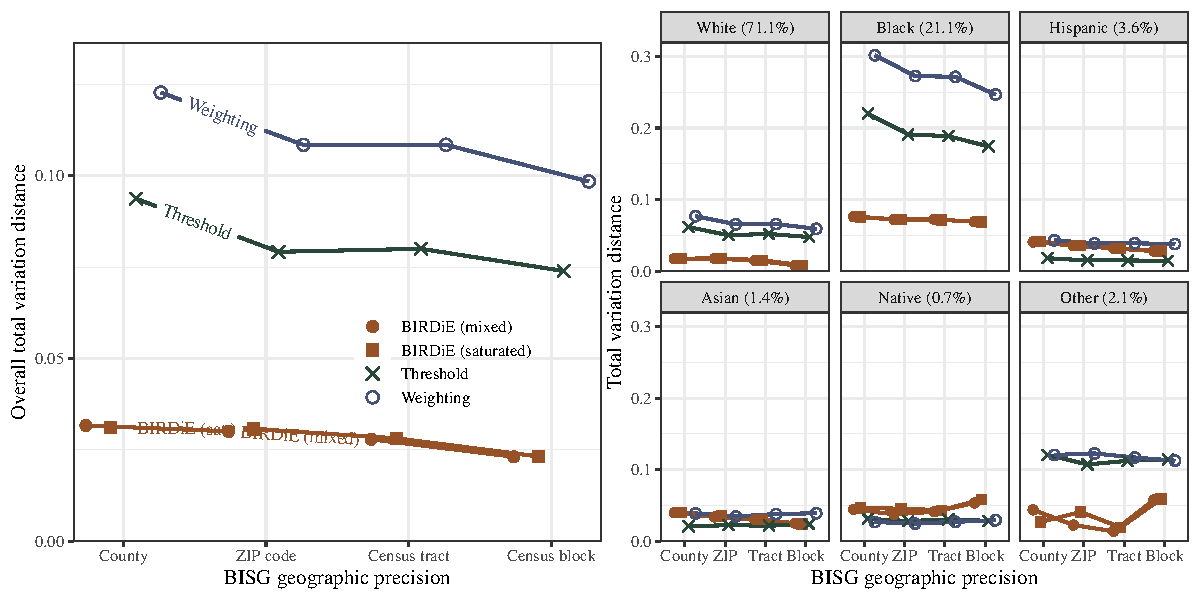
\includegraphics[width=\textwidth]{../paper/figures/nc_tv.pdf}

\end{frame}

\begin{frame}

  \frametitle{Small Area Estimation}

 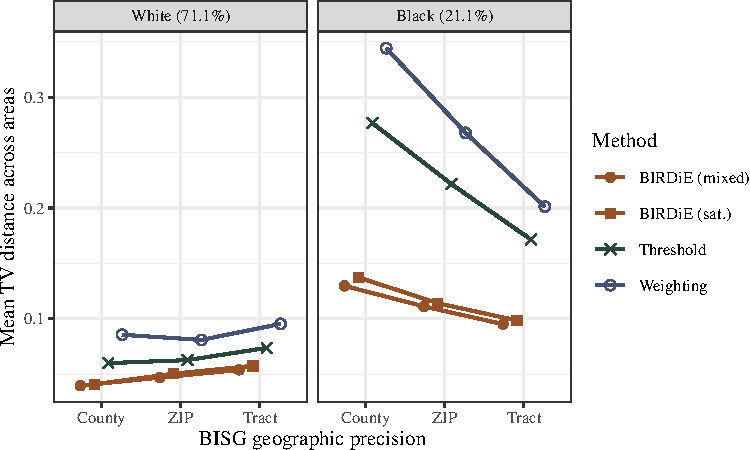
\includegraphics[width=\textwidth]{../paper/figures/nc_smallarea.pdf}


\end{frame}

\begin{frame}

  \frametitle{Improved Race Probabilities}

 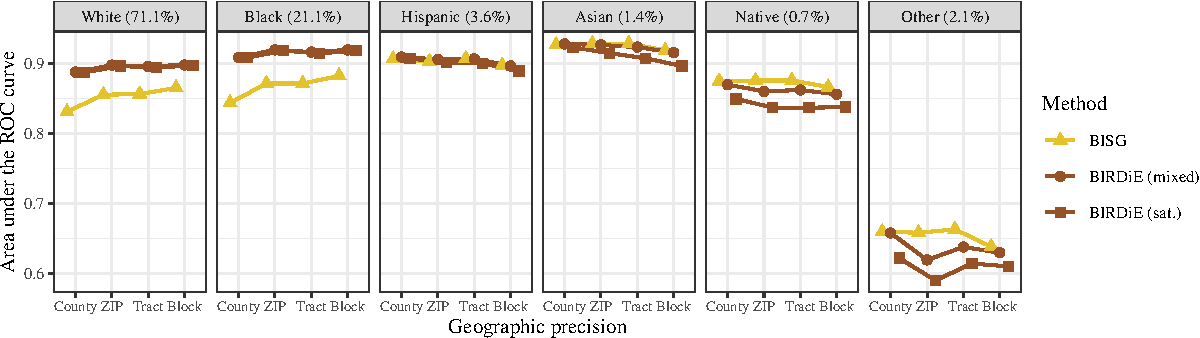
\includegraphics[width=\textwidth]{../paper/figures/nc_roc.pdf}


\end{frame}

\begin{frame}

  \frametitle{Estimates Conditional on an Additional Variable}

 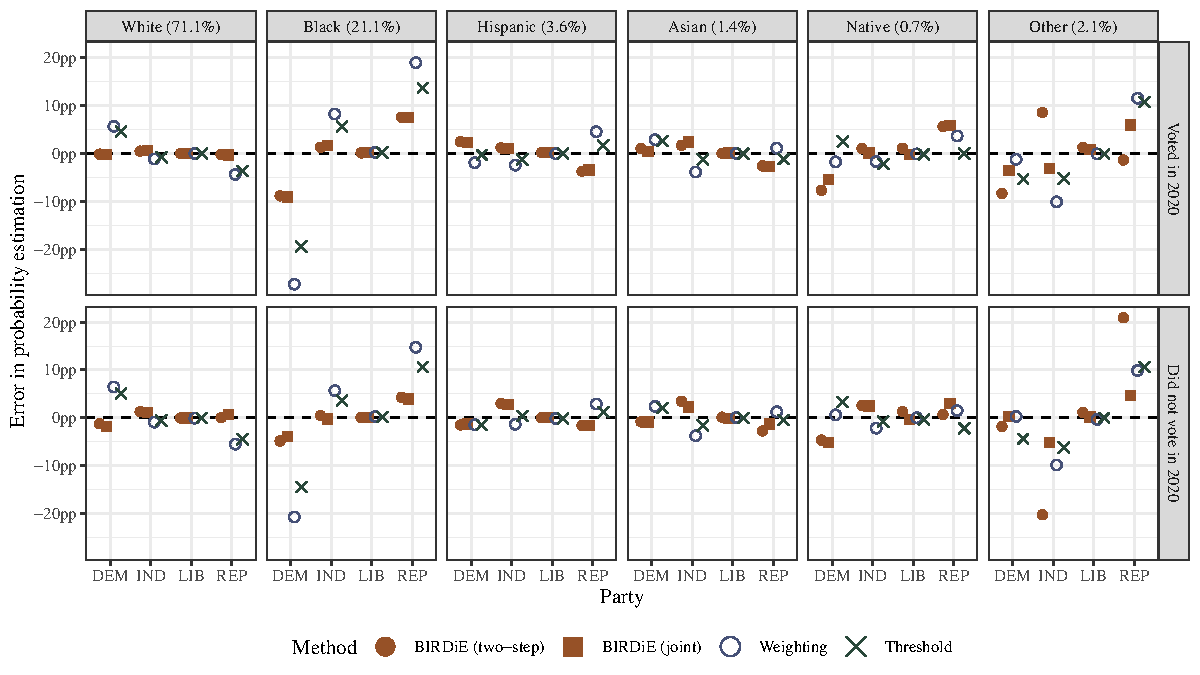
\includegraphics[width=\textwidth]{../paper/figures/nc_addlcov_error.pdf}


\end{frame}

\begin{frame}

  \frametitle{Robustness Analysis}

  \begin{itemize}
  \item Surname groups from 1930 Census  
  \item Added 3,000 Asian surnames to account for more recent
    immigration
    \vfill
  \item Correlation between BIRDiE residuals and nine surname groups
    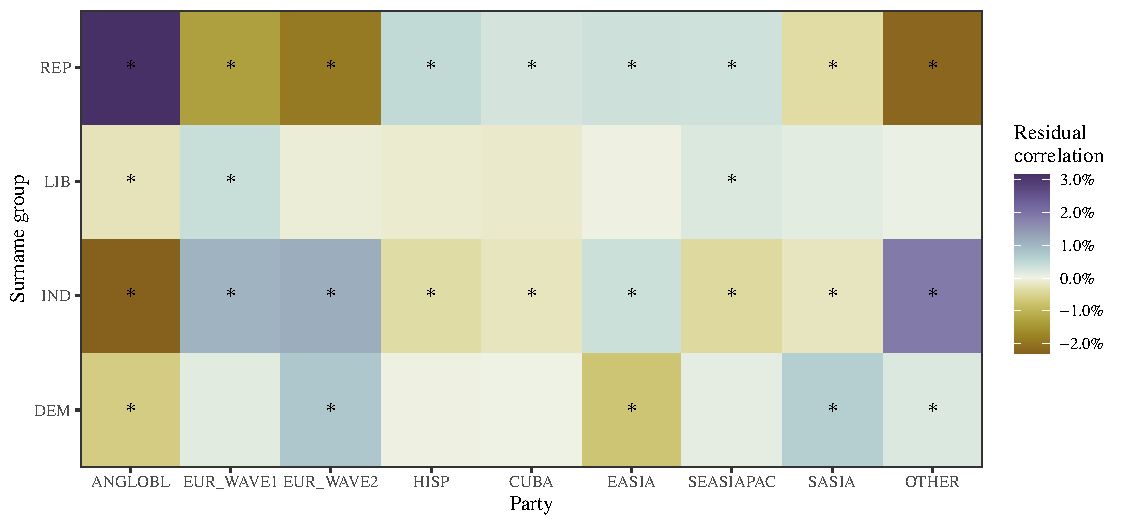
\includegraphics[width=0.9\textwidth]{../paper/figures/nc_sens_grp.pdf}

  \item Including these in BIRDiE does not substantially alter the estimates 
  \end{itemize}

\end{frame}


\begin{frame}

  \frametitle{Concluding Remarks}

  \begin{itemize}
  \item BIRDiE
    \begin{itemize}
    \item New identification assumption
    \item Flexible modeling with scalable estimation
    \item Improved BISG race probabilities
    \item Sensitivity analysis
    \end{itemize}
    \vfill

  \item Future work
    \begin{itemize}
    \item additional empirical validations: understanding bias
    \item better use of auxiliary information in sensitivity analysis
    \item make BIRDiE more robust to small bias in BISG probabilities

    \end{itemize}
  \end{itemize}

  \vfill
  \onslide<10->{\begin{center}
    The paper is available at
    \alert{\url{https://imai.fas.harvard.edu/research/birdie.html}} \\
    \vfill
    The software is available at \\
    \alert{\url{https://corymccartan.com/birdie/}} 
  \end{center}}
  \vspace{-.7in}
  \begin{flushright}
     
\includegraphics[scale=0.165]{../man/figures/logo.png}
  \end{flushright}
\end{frame}


\end{document}